\chapter{Технологическая часть}

В данном разделе были рассмотрены средства, использованные для разработки, а также приведены коды реализованных алгоритмов.

\section{Средства реализации}

Выбор языка программирования C\# для реализации курсовой работы обусловлен его техническими возможностями и поддержкой объектно-ориентированного программирования. Также обеспечивание высокой производительности благодаря компиляции в промежуточный язык и широкая документация упрощают процесс разработки, а автоматическое управление памятью снижает риск ошибок, связанных с утечками ресурсов. 


\section{Программный интерфейс}

На рисунке~\ref{images:morning} представлен графический интерфейс программы.

\begin{figure}[H]
    \centering
    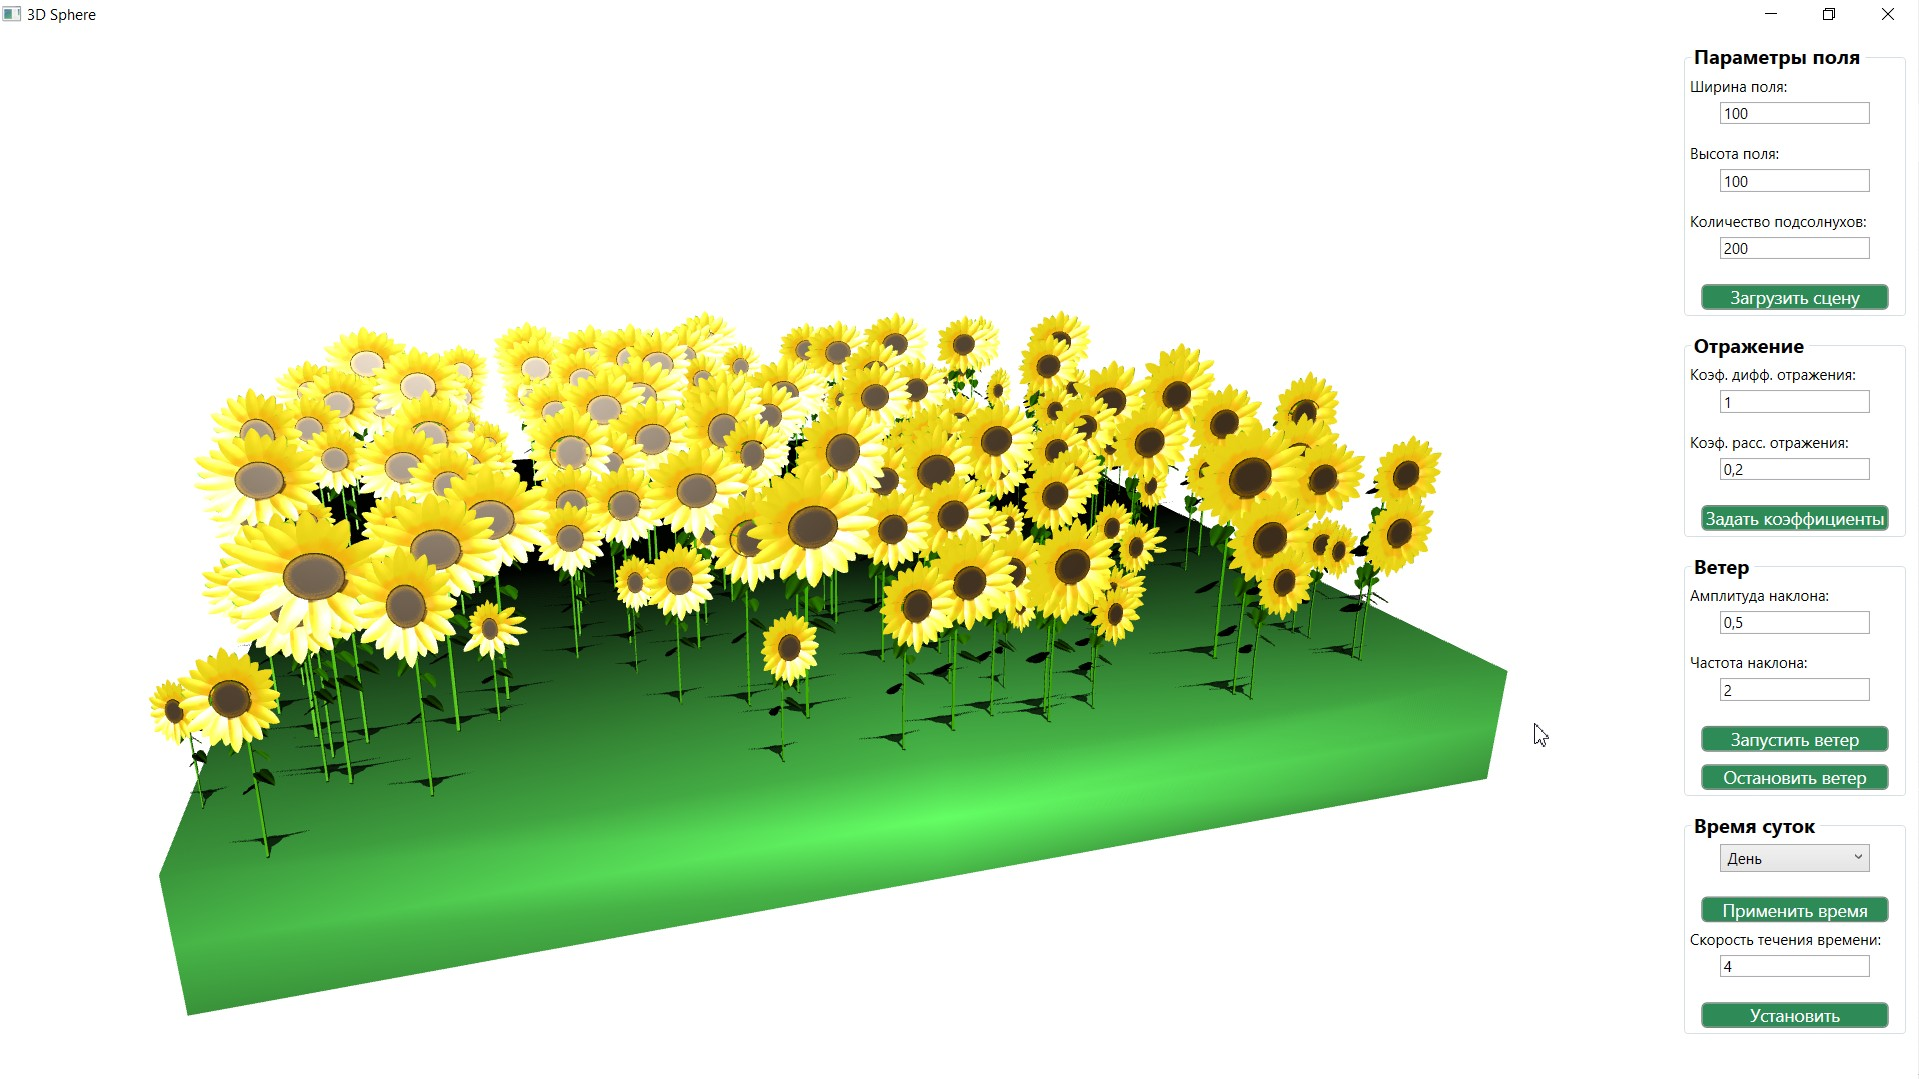
\includegraphics[width=150mm]{images/morning}
    \caption{Графический интерфейс программы.}
    \label{images:morning}
\end{figure}

На рисунках~\ref{images:Morning},~\ref{images:Day},~\ref{images:Evening},~\ref{images:Night} представлены результаты работы программы при различных заданных пользователем временах суток: утро, день, вечер и ночь соответственно.

\begin{figure}[H]
    \centering
    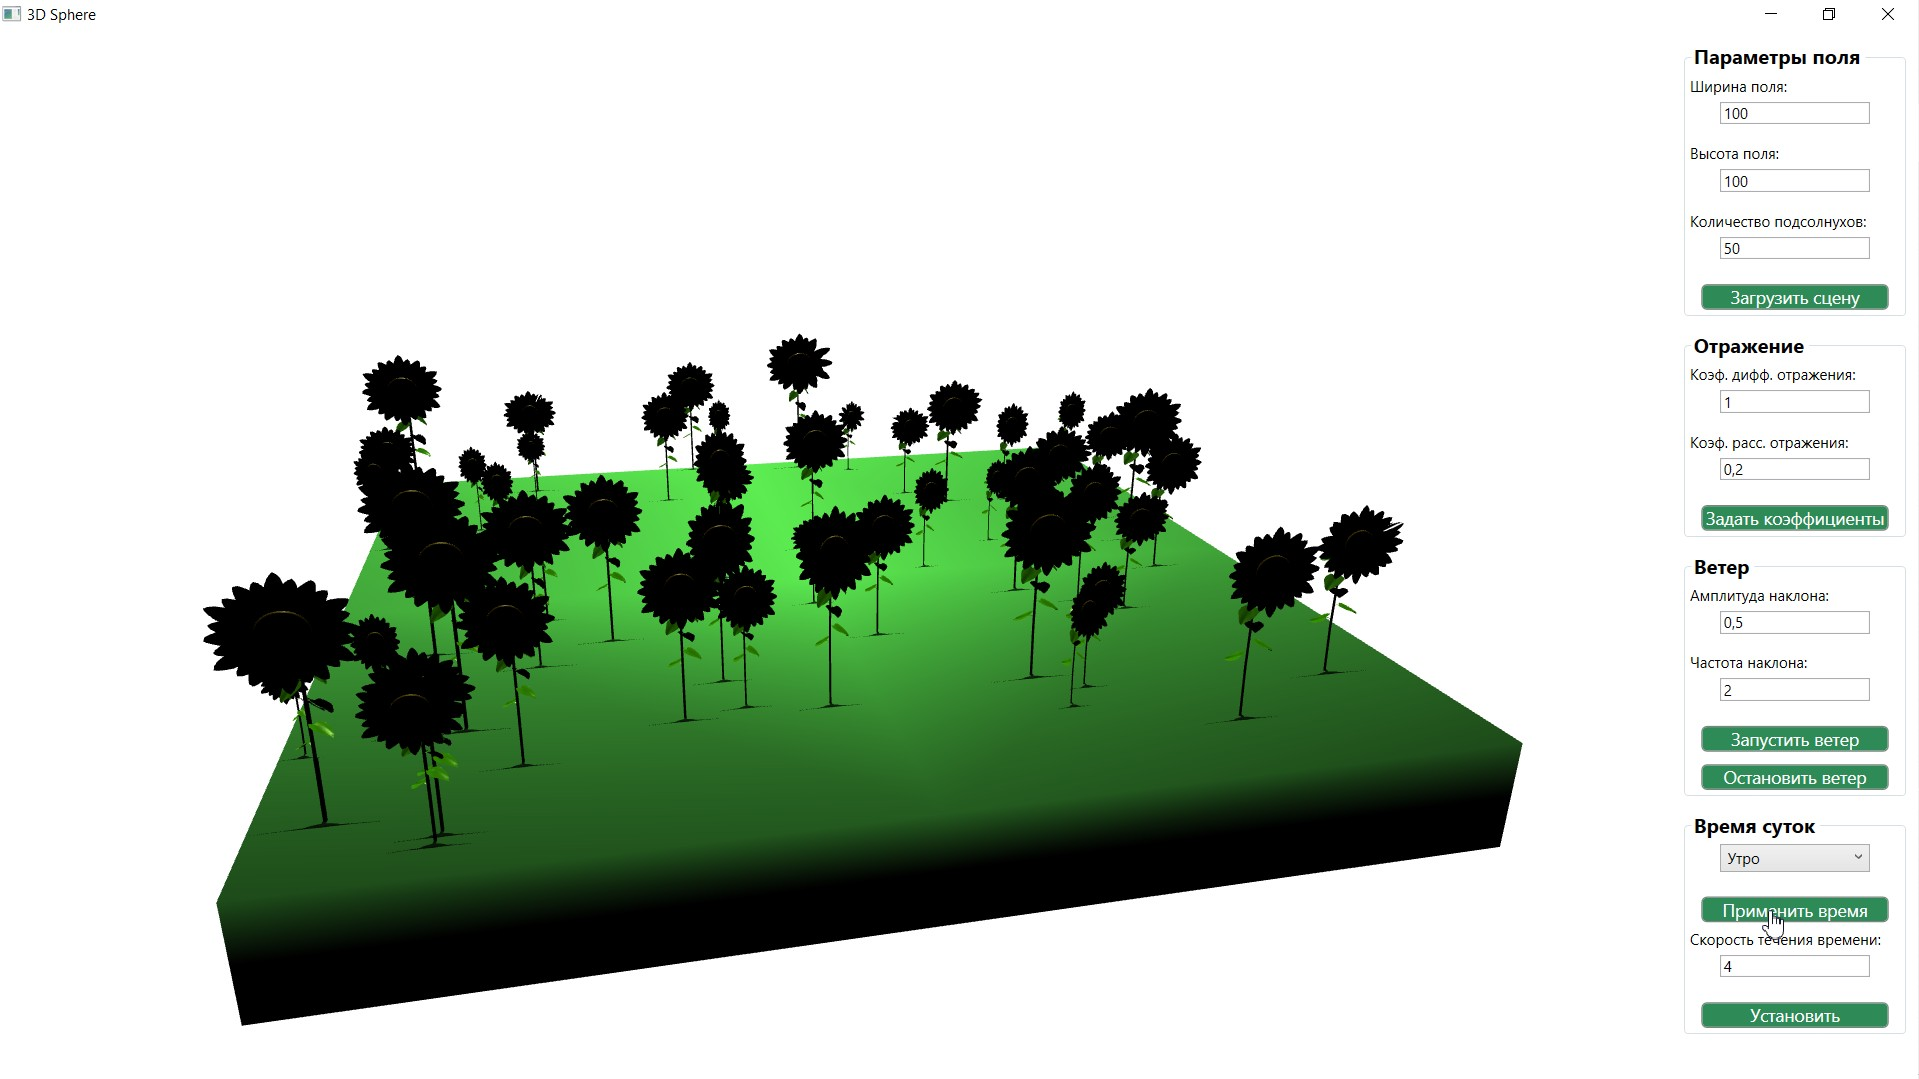
\includegraphics[width=150mm]{images/morning_50}
    \caption{Графический интерфейс программы.}
    \label{images:Morning}
\end{figure}

\begin{figure}[H]
    \centering
    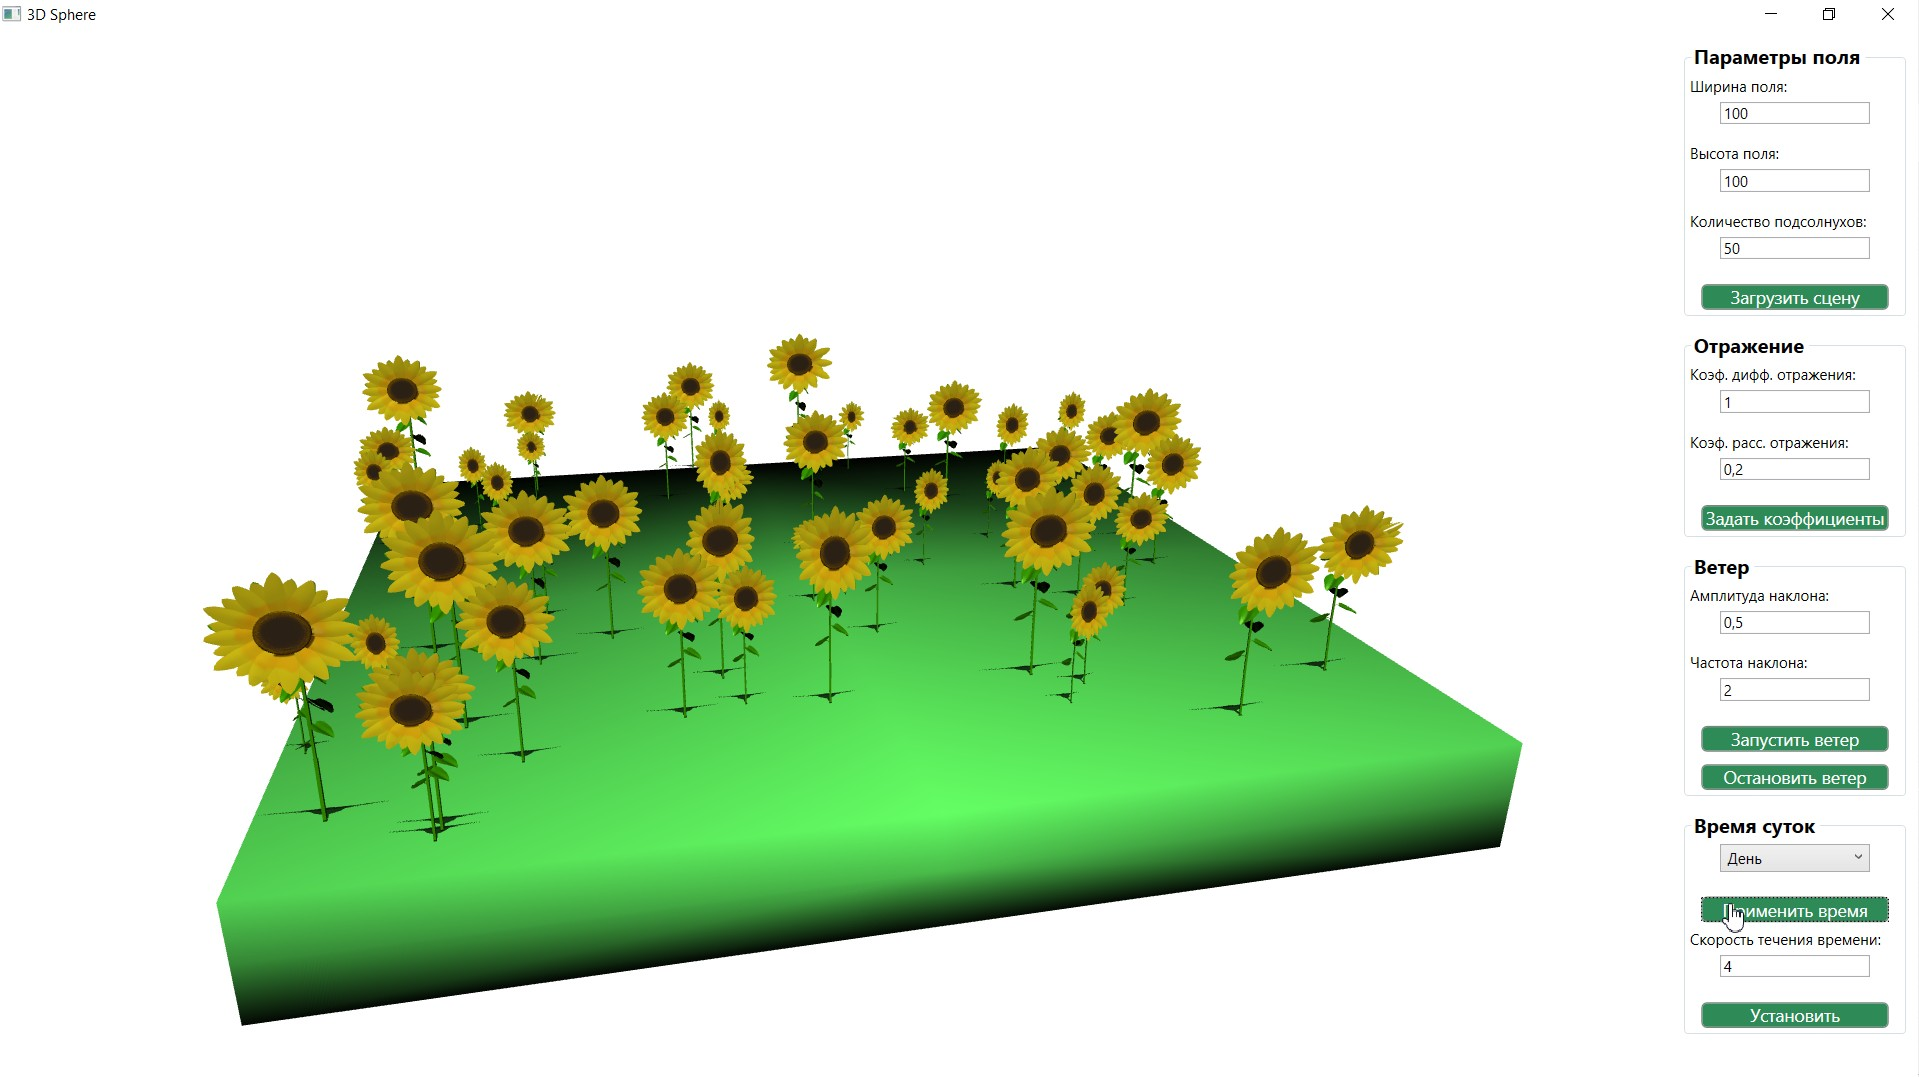
\includegraphics[width=150mm]{images/day_50}
    \caption{Графический интерфейс программы.}
    \label{images:Day}
\end{figure}

\begin{figure}[H]
    \centering
    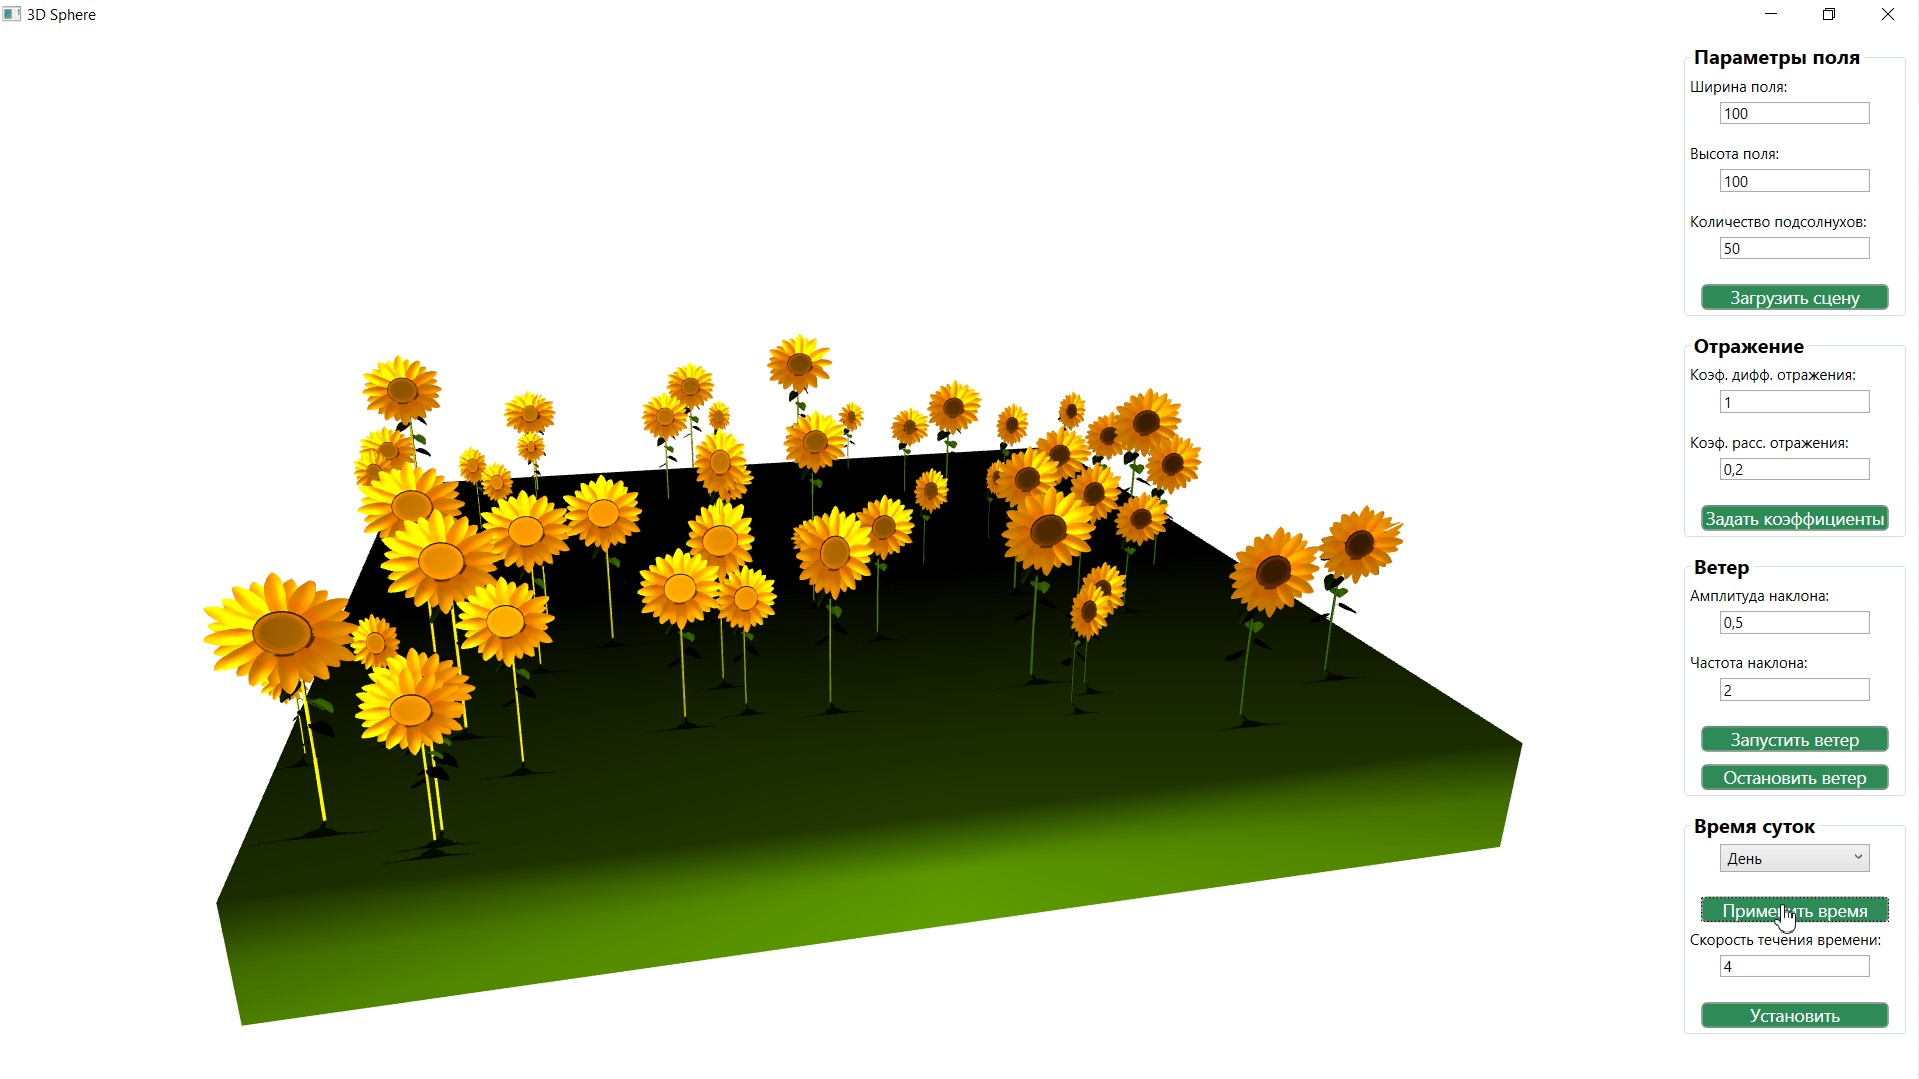
\includegraphics[width=150mm]{images/evening_50}
    \caption{Графический интерфейс программы.}
    \label{images:Evening}
\end{figure}

\begin{figure}[H]
    \centering
    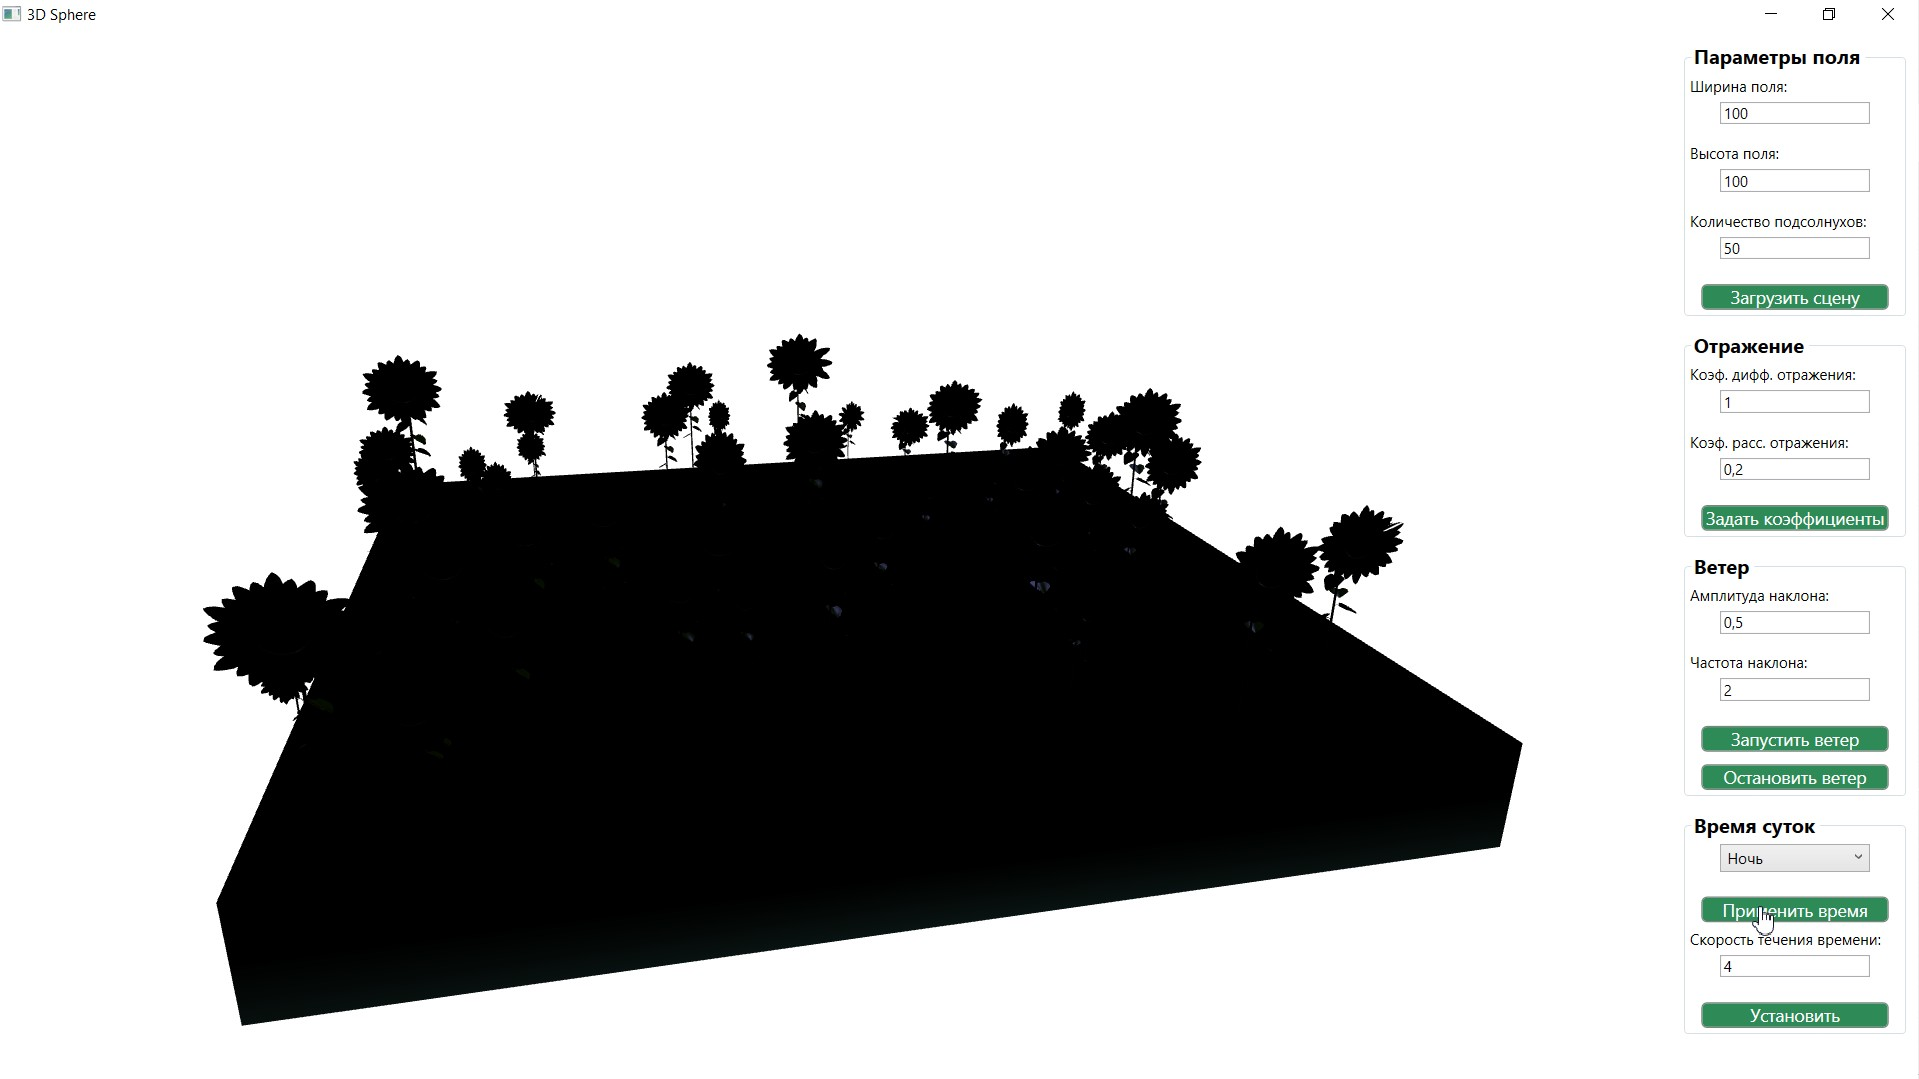
\includegraphics[width=150mm]{images/night_50}
    \caption{Графический интерфейс программы.}
    \label{images:Night}
\end{figure}

\subsection{Реализация алгоритмов}

В листинге~\ref{lst:l_iteration} представлен алгоритм применения ветра к модели.
\begin{center}
\begin{lstlisting}[caption={Алгоритм применения ветра к модели}, label={lst:l_iteration}]
private Transform3D CalculateTransform(GeometryModel3D geometryModel)
        {
            var meshGeometry = geometryModel.Geometry as MeshGeometry3D;
            if (meshGeometry == null) return geometryModel.Transform;

            var transform = new Transform3DGroup();
            transform.Children.Add(_originalTransforms[geometryModel]);

            double windStrength = _amplitude * Math.Sin(_timeElapsed * _frequency * 2 * Math.PI);

            var boneTransforms = new Dictionary<Bone, Matrix3D>();
            
            var bone00 = _bones.FirstOrDefault(b => b.Name == "root");
            var bone01 = _bones.FirstOrDefault(b => b.Name == "Sunflower01");
            var bone02 = _bones.FirstOrDefault(b => b.Name == "Sunflower02");
            var bone03 = _bones.FirstOrDefault(b => b.Name == "Sunflower03");
            var bone04 = _bones.FirstOrDefault(b => b.Name == "Sunflower04");
            var bone05 = _bones.FirstOrDefault(b => b.Name == "Sunflower05");
            var bone5 = _bones.FirstOrDefault(b => b.Name == "Sunflower5");

            ApplyBoneTransform(bone00, null, windStrength, boneTransforms);
            ApplyBoneTransform(bone01, bone00, windStrength, boneTransforms);
            ApplyBoneTransform(bone02, bone01, windStrength, boneTransforms);
            ApplyBoneTransform(bone03, bone02, windStrength, boneTransforms);
            ApplyBoneTransform(bone04, bone03, windStrength, boneTransforms);
            ApplyBoneTransform(bone05, bone04, windStrength, boneTransforms);
            ApplyBoneTransform(bone5, bone05, windStrength, boneTransforms);
            
            foreach (var bone in _bones)
            {
                if (boneTransforms.ContainsKey(bone))
                {
                    ApplyRotationToBone(meshGeometry, bone, boneTransforms[bone]);
                }
            }
            
            var newMeshGeometry = new MeshGeometry3D
            {
                Positions = meshGeometry.Positions,
                TriangleIndices = meshGeometry.TriangleIndices,
                Normals = meshGeometry.Normals,
                TextureCoordinates = meshGeometry.TextureCoordinates
            };

            geometryModel.Geometry = newMeshGeometry;
            return transform;
        }
\end{lstlisting}
\end{center}

В листинге~\ref{lst:l_iteration} представлен метод для применения вращения к вершинам кости.
\begin{center}
\begin{lstlisting}[caption={Метод для применения вращения к вершинам кости}, label={lst:l_iteration}]
private void ApplyBoneTransform(Bone bone, Bone parentBone, double windStrength, Dictionary<Bone, Matrix3D> boneTransforms)
        {
            if (bone == null) return;

            double angle = windStrength * GetBoneMultiplier(bone.Name);
            var localRotation = new RotateTransform3D(new AxisAngleRotation3D(new Vector3D(1, 0, 0), angle)).Value;

            
            if (parentBone != null && boneTransforms.ContainsKey(parentBone))
            {
                boneTransforms[bone] = localRotation * boneTransforms[parentBone];
            }
            else
            {
                boneTransforms[bone] = localRotation;
            }
        }
\end{lstlisting}
\end{center}

В листинге~\ref{lst:l_iteration} представлен алгоритм преобразования координат вершин трехмерной модели, связанных с определенной "костью" (bone), с использованием заданной матрицы поворота.
\begin{center}
\begin{lstlisting}[caption={Алгоритм преобразования координат вершин модели}, label={lst:l_iteration}]
private void ApplyRotationToBone(MeshGeometry3D meshGeometry, Bone bone, Matrix3D rotationMatrix)
        {
            foreach (var vertexIndex in bone.ConnectedVertices)
            {
                if (vertexIndex < meshGeometry.Positions.Count)
                {
                    var originalPosition = meshGeometry.Positions[vertexIndex];
                    var newPosition = rotationMatrix.Transform(originalPosition);
                    meshGeometry.Positions[vertexIndex] = newPosition;
                }
            }
        }
\end{lstlisting}
\end{center}


В листинге~\ref{lst:test_count} представлен тест для исследования времени загрузки сцены в зависимости от количества подсолнухов.
\begin{center}
\begin{lstlisting}[caption={Тест для исследования времени загрузки сцены в зависимости от количества подсолнухов}, label={lst:test_count}]
public void TestSunflowerFieldLoading(object sender, RoutedEventArgs e)
        {
            double width = 100.0;
            double height = 100.0;

            for (int countSunflowers = 1; countSunflowers <= 401; countSunflowers += 20)
            {
                ClearScene();

                Stopwatch stopwatch = Stopwatch.StartNew();

                _sunflowerField = new SunflowerField(width, height, _fieldPath, countSunflowers, _sunflowerModelPath, _sunflowerTexturePath);
                
                stopwatch.Stop();

                Console.WriteLine($"countSunflowers: {countSunflowers}, Time: {stopwatch.Elapsed.TotalMilliseconds} ms");
            }
        }
\end{lstlisting}
\end{center}


В листинге~\ref{lst:test_w_h} представлен тест для исследования времени загрузки сцены в зависимости от длины и ширины поля.
\begin{center}
\begin{lstlisting}[caption={Тест для исследования времени загрузки сцены в зависимости от длины и ширины поля}, label={lst:test_w_h}]
public void TestSunflowerFieldLoadingWithVariableSceneSize(object sender, RoutedEventArgs e)
        {
            int countSunflowers = 50; 

            for (double width = 10; width <= 2010; width += 200)
            {
                for (double height = 10; height <= 2010; height += 200)
                {
                    ClearScene();

                    Stopwatch stopwatch = Stopwatch.StartNew();

                    _sunflowerField = new SunflowerField(width, height, _fieldPath, countSunflowers, _sunflowerModelPath, _sunflowerTexturePath);

                    stopwatch.Stop();

                    Console.WriteLine($"Width: {width}, Length: {height}, Time downloading {stopwatch.Elapsed.TotalMilliseconds} ms");
                }
            }
        }
\end{lstlisting}
\end{center}


В листинге~\ref{lst:test_cpu} представлен тест для исследования загруженности процессора при включенном ветре и различном количестве подсолнухов.
\begin{center}
\begin{lstlisting}[caption={Тест для исследования загруженности процессора при включенном ветре и различном количестве подсолнухов.}, label={lst:test_cpu}]
public void TestWindPerformance(object sender, RoutedEventArgs e)
        {
            double width = 100.0;
            double height = 100.0;
            
            for (int countSunflowers = 1; countSunflowers <= 401; countSunflowers += 20)
            {
                ClearScene();

                _sunflowerField = new SunflowerField(width, height, _fieldPath, countSunflowers, _sunflowerModelPath, _sunflowerTexturePath);

                _sunflowerField.StartWind(amplitude: 0.1, frequency: 0.5);
                double cpuUsage = MeasureCpuUsage(duration: 10000); 

                _sunflowerField.StopWind();

                Console.WriteLine($"countSunflowers: {countSunflowers}, CPU usage : {cpuUsage:F2}%");
            }
        }
\end{lstlisting}
\end{center}

Все тесты были пройдены успешно.

\section*{Вывод}

В технологической части была рассмотрена реализация программного обеспечения для моделирования поля подсолнухов с учетом ветра. Тестирование показало эффективность программы, а также выявило возможности для дальнейшей оптимизации. 